\documentclass[../main.tex]{subfiles}
%\graphicspath{{\subfix{images/}}}

\begin{document}

Computational complexity theory is the foundation of computational security of modern cryptography by allowing one to emphasize the security of a cryptosystem by drawing an efficient reduction from a computationally hard problem (that either has been proved or is believed with high confidence to be unsolvable in a reasonable time, e.g., polynomial time). That being said, a cryptosystem that is provably secure is still vulnerable to real-world attacks, depending on what threat model was considered, how close to reality the underlying security definitions and assumptions are and so on. 

In this chapter, we start by introducing some basic definitions in computational complexity theory, then go on to talk about inapproximability, which are variants of the standard decision and optimization problems and commonly used to prove the computational security of cryptosystems. We then introduce gap problems, which are generalization of decision problems and proving their hardness is a useful technique of proving inapproximability. We finish the chapter by briefly introducing \citet{ajtai1996generating}'s worst-case to average-case reduction. Ajtai's work is considered as the first published average-case problem whose hardness is based on the worst-case hardness of some well-known lattice problems.

\subsection{Basic time complexity classes}

The following concepts are introduced under the assumption that a general purpose computer is of the form of a \textit{Turing machine}. The primary reference book of this subsection is \cite{sipser2013introduction}. 

A \textit{language (or decision problem)} 
\reversemarginpar
\marginnote{\textit{Decision problem}}
is a set of strings that are decidable by a Turing machine. We use $\Sigma$ to denote the alphabet and $\Sigma^*$ to denote the set of all strings over the alphabet $\Sigma$ of all lengths. A special case is when $\Sigma=\{0,1\}$ and $\Sigma^*=\{0,1\}^*$ is the set of all strings of $0$s and $1$s of all lengths. In this case, a language $A=\{x \in \{0,1\}^* \mid f(x)=1\}$, where $f:\{0,1\}^* \rightarrow \{0,1\}$ is a \textit{Boolean function}.

Let $M$ be a deterministic Turing machine that halts on all inputs. We measure the 
\reversemarginpar
\marginnote{\textit{Time complexity}}
\textbf{time complexity} or \textbf{running time} of $M$ by the function $t:\N \rightarrow \N$, where $t(n)$ is the maximum number of steps that $M$ takes on any input of length $n$. Generally speaking, $t(n)$ can be any function of $n$ and the exact number of steps may be difficult to calculate, so we often just analyse $t(n)$'s \textbf{asymptotic behaviour} by taking its leading term, denoted by $O(t(n))$. We also relax its codomain by letting $t:\N \rightarrow \R^+$ be a non-negative real valued function. 

It is worth mentioning that when analysing the time complexity of a function, we often consider its time complexity in the worst case, i.e., the longest running time of all inputs of a particular length $n$. At the end of this chapter, we will emphasize the importance of the worst-case complexity in the proof of security of modern cryptosystems. We will give a clue of how this was achieved by \citet{ajtai1996generating} through an average-case to worst-case reduction.

\begin{definition}
The \textbf{time complexity class},
\reversemarginpar
\marginnote{\textit{Time complexity class}}
$\mathbf{TIME(t(n))}$, is defined as the set of all languages that are decidable by a Turning machine in time $O(t(n))$.
\end{definition}

Obviously, $t$ can be any function, e.g., logarithm, polynomial, exponential, etc. In practice, polynomial differences in running time are considered to be much better than exponential differences due to the super fast growth rate of the latter. For this reason, we separate languages into different classes according to their worst case running time on a deterministic single-tape Turing machine. 

\begin{definition}
\textbf{P} \index{time complexity class!P}
\reversemarginpar
\marginnote{\textit{P}}
is the class of languages that are decidable in polynomial time by a deterministic single-tape Turing machine, i.e., % for a constant $k$, 
\begin{equation*}
    P = \bigcup_{k \in \N} \it{TIME}(n^k).
\end{equation*}
\end{definition}

Some problems are computationally hard, so cannot be decided by a deterministic single-tape Turing machine in polynomial time. But given a possible solution, sometimes we can efficiently \textit{verify} whether or not the solution is genuine. The length of the solution has to be polynomial in the length of the input string length, for otherwise the verification process cannot be done efficiently. Based on the ability to efficiently verify, we can define the complexity class NP. 

\begin{definition}
\textbf{NP} \index{time complexity class!NP}
\reversemarginpar
\marginnote{\textit{NP}}
is the class of languages that can be verified in polynomial time.
\end{definition}

\iffalse % KS: we don't seem to need this definition in the rest of the paper
An alternative definition of NP is based on a \textbf{non-deterministic Turing machine}.
\reversemarginpar
\marginnote{\textit{NDTM}}
We can define the time complexity class $NTIME(t(n))$ for a non-deterministic Turing machine as the set of all languages that are decidable by a non-deterministic Turing machine. 

\begin{definition}
\textbf{NP} is the class of languages that are decidable in polynomial time by a non-deterministic Turing machine, i.e., % for a constant $k$
\begin{equation*}
    NP=\bigcup_{k \in \N} \it{NTIME}(n^k).
\end{equation*}
\end{definition}
\fi

Sometimes, a problem can be solved by reducing it to another problem, whose solution can be found relatively easier, provided the reduction between the two problems is efficient. For example, a polynomial time reduction is often acceptable.   
%The efficient reduction can be formally defined as the next. 

\begin{definition}
A language $A$ is \textbf{polynomial time reducible} 
\reversemarginpar
\marginnote{\textit{PT reduction}}
to another language $B$, written as $A \le_P B$, if a polynomial time computable function $f:\Sigma^* \rightarrow \Sigma^*$ exists, where for every $w$, 
\begin{equation*}
    w \in A \iff f(w) \in B.
\end{equation*}
\end{definition}

A polynomial time reduction $A \le_P B$ implies $A$ is no harder than $B$, so if $B \in \text{P}$ then $A \in \text{P}$. Based on this reduction, we can define another complexity class. 

\begin{definition}
A language $B$ is \textbf{NP-complete} \index{time complexity class!NP-complete}
\reversemarginpar
\marginnote{\textit{NP-complete}}
if it is in NP and every problem in NP is polynomial time reducible to $B$. 
\end{definition}
Essentially, we are saying that NP-complete is the set of the hardest problems in NP. There are, however, hard problems that are not in NP such as an \textbf{optimization problem}. Given a solution of an optimization problem, it is often not trivial to verify the solution is optimal among all the answers, so this type of problems are not polynomial time verifiable and hence not in NP. For these problems, we can define a similar complexity class as NP-complete but without requiring their solutions to be polynomially checkable. 

\begin{definition}
A language is \textbf{NP-hard} \index{time complexity class!NP-hard}
\reversemarginpar
\marginnote{\textit{NP-hard}}
if every problem in NP is polynomial time reducible to it. 
\end{definition}
 
The two terms NP-complete and NP-hard are sometimes used  interchangeably because an optimization problem can also be formed as a decision problem. For example, instead of asking for the shortest route from the \textit{travelling salesman problem}, we can ask whether there exists a route that is shorter than a threshold. 

Many optimization problems are NP-hard, which means there is no polynomial time solution under the assumption $\text{P}\neq \text{NP}$. Hence, when an answer for an NP-hard problem is needed, the fallback is to use an approximation algorithm to compute a near-optimal solution that is within an acceptable range. 
% However, giving the best possible answers is not in the most interest of cryptographers. Instead, 
For a NP-hard problem, it is sometimes easier to build a cryptosystem based on its approximated version rather than the NP-hard problem itself. For this reason, cryptographers are concerned about whether or not an optimization problem is hard to be approximated within a certain range. % for an approximated answer.
This brings us to the study of the hardness of approximation or inapproximability in the next subsection. 

\subsection{Hardness of approximation}
\label{subsection:gapProb}

An optimization problem aims at finding the optimum result of a computational problem. This optimum result can either be the maximum or minimum of some value. Throughout this section, we focus on minimization problems only. The same results also hold for maximization problems. \footnote{Lecture 18: \textit{Gap Inapproximability}, 6.892 \textit{Algorithmic Lower Bounds: Fun with Hardness Proofs} (Spring 2019), Erik Demaine, available at
 \url{http://courses.csail.mit.edu/6.892/spring19/lectures/L18.html}} 
In the previous section, we said an optimization problem can be made into a decision problem by comparing the solution with a threshold. More formally, it is defined as the next. 

\begin{definition}
An \textbf{NP-optimization} (NPO) problem
\reversemarginpar
\marginnote{\textit{NPO}}
is an optimization problem such that 
\begin{itemize}
    \item all instances and solutions can be recognized in polynomial time,
    \item all solutions have polynomial length in the length of the instance,
    \item all solution's costs can be computed in polynomial time.
\end{itemize}
\end{definition}
% NPO is the class of all NP-optimization problems. 
For a minimization problem in NPO, its decision version asks ``Is $OPT(x) \le q$?'', where $OPT(x)$ is the unknown optimal solution (or its cost, we use interchangeably) to the instance $x$. For example, in the \textit{maximum clique} problem, an instance is a graph, an optimal solution is the maximum clique in the given graph and its cost is the clique size. Given an NPO problem, its decision version is an NP problem, so NPO is an analogy of NP but for optimization problems. On the other hand, PO (P-optimization) problem is the set of optimization problems whose decision versions are in P, such as finding the shortest path. 

\begin{definition}
An algorithm $ALG$ for a minimization problem is called \textbf{$c$-approximation algorithm} \index{$c$-approximation} for $c \ge 1$
\reversemarginpar
\marginnote{\textit{$c$-approx}}
if for all instances $x$, it satisfies 
\begin{equation}
    \frac{cost(ALG(x))}{cost(OPT(x))} \le c.
\end{equation}
\end{definition}
The ratio $c$ is not necessarily a constant, it can be any function of the input size, i.e., $c=f(n)$ for an arbitrary function $f(\cdot)$. Practically, we prefer a near optimal solution $ALG(x)$ such that the ratio $c$ is as small as possible or at least does not grow quickly in the input size. This, however, may not be possible for some problems such as the maximum clique problem, whose best possible ratio is $O(n^{1-\epsilon})$ for small $\epsilon > 0$. 
From a provable security's perspective, the smaller the ratio $c$ is, the harder the c-approximation problem is. This leads to a cryptosystem with higher security because it requires more time and computational resources for an attacker to break the system. 

For a given $c=f(n)$, there are different ways of proving $c$-approximating a problem is hard. One way is by proving a c-gap problem is hard, which is in direct analogy to the c-approximation problem in hand. This way, if the gap problem is hard, then the $c$-approximation problem is also hard.  

\begin{definition}
For a minimization problem, a \textbf{$c$-gap problem} \index{$c$-gap problem}
\reversemarginpar
\marginnote{\textit{$c$-gap}}
(where $c > 1$) distinguishes two cases for the optimal solution $OPT(x)$ of an instance $x$ and a given $k$ as follows:
\begin{itemize}
    \item $x$ is an YES instance if $OPT(x) \le k$,
    \item $x$ is an NO instance if $OPT(x) > c\cdot k$.
\end{itemize}
\end{definition}

The value $k$ is a given input. For example, in the $c$-gap version of the shortest vector problem, we can set $k=\lambda_1(L)$ to be the shortest vector in a given lattice $L$. Intuitively, a $c$-gap problem is a decision problem where the unknown optimal solution $OPT$ of the corresponding optimization problem is mapped to the opposite side of a gap. It is, however, different from a decision problem in the sense that there is a gap between $k$ and $c\cdot k$.

\iffalse % KS: Promise Problems don't seem to be needed in the rest of the paper
To be more precise, a $c$-gap problem is a promise problem. A \textbf{promise problem}
is a generalization of a decision problem, where only a subset of the entire input space is considered. Alternatively, we can think of the algorithm is only defined for a subset of the entire input space. For example, instead of taking the set of all graphs as inputs, a promise problem may only consider connected graphs. Hence, it is the union of two disjoint subsets, one contains all the YES instances and the other contains all the NO instances. These two classes of instances make the entire set of connected graphs. But if a given graph is not connected, the algorithm for solving the promise problem can return any output or may not even halt. It is named ``promise'' because all inputs are promised to be on either side of the gap, nothing falls in between.\footnote{See Erik Demaine's MIT lecture notes for more details. \url{http://courses.csail.mit.edu/6.892/spring19/lectures/L18.html}}
\fi

The connection between c-gap and c-approximation problems is that if a c-gap problem is proved to be hard, then the corresponding c-approximation problem is also hard. 
\reversemarginpar
\marginnote{\textit{$c$-gap implies inapprox }}
In other words, there is a reduction from a c-gap problem to a c-approximation problem. The proof is straightforward. 
Assuming the problem can be c-approximated in polynomial time by an algorithm $A$, so for an input $x$ we have $OPT(x) \le A(x) \le c\cdot OPT(x)$.
If $x$ is a YES instance of the gap problem, then 
\begin{equation*}
    OPT(x) \le k \implies A(x) \le c \cdot OPT(x) \le c\cdot k.
\end{equation*}
If $x$ is a NO instance, then 
\begin{equation*}
    OPT(x) > c \cdot k \implies A(x) > c \cdot k.
\end{equation*}
Either way the instance $x$ can be distinguished easily using the decision procedure $A(x) \leq c\cdot k$. %, so it solves the $c$-gap problem. 

Gap and approximation lattice problems are the foundation of provable security for latticed-based cryptosystems. We will see more of these problems in \Cref{section:lattice theory} and some of their cryptographical applications in the hardness proofs of the short integer solution problem, learning with error problem and ring learning with error problem. 

\iffalse
\subsection{One way function}

We now introduce one-way functions which will be mentioned in the next section for worst-case to average-case reduction. 

One-way functions are essential for the security of cryptographic primitives. Intuitively, a one-way function is a function $f: \{0,1\}^n \rightarrow \{0,1\}^n$ that can be computed in polynomial time, but hard to be inverted.

In particular, if $f$ is a one-way function and injective (or one-to-one), then $f$ is a \textbf{one-way permutation}.

Formal definition will be filled in, see Chapter 7.1 in \citep{katz2014introduction} or Chapter 10.6 in \citep{sipser1996introduction}, may need to introduce the concept of probabilistic polynomial-time algorithm, see Chapter 10.2 in \citep{sipser1996introduction}.

The existence of one-way functions is an open problem. That is, no one can prove the existence of one-way functions unconditionally. 

Some examples of one-way functions are prime factorization (complexity class is known), subset sum problem (known to be NP-complete), discrete logarithm problem and permutations. 
\fi 



\subsection{Average-case to worst-case hardness}
\label{subsec:averagecasehard}

So far, we have introduced the time complexity classes P and NP in the worst case scenario. That is, the longest running time over all inputs at a given input length. A problem that is hard to be solved in polynomial time in the worst case is known as worst-case hard. There is another related concept called average-case hardness, \index{average-case hardness} which is stronger than worst-case hardness, in the sense that the former implies the latter but not vice versa. To finish section, we briefly discuss the critical role of average-case hard problems for cryptography and how they can be constructed by a worst-case to average-case reduction \index{worst-case to average-case} that was achieved in \citet{ajtai1996generating}. 

%Average-case hardness is a stronger assumption than worst-case hardness, as if a problem is average-case hard then it must be worst-case hard, but not vice versa. For that matter, it is preferable to build a cryptosystem, whose security is based on a weaker assumption (i.e., worst-case hardness) rather than a stronger assumption (i.e., average-case hardness). Intuitively, this also makes sense. Because if an attacker is able to solve a decent number of instances of an average-case hard problem, he may claim that the problem is not hard and hence any cryptosystem that is build upon it is not safe. On the other hand, the attacker cannot make such a claim against a worst-case hard problem unless he has solved every instance of the problem. 

Without going into the details of average-case problems, we state some remarks (Chapter 18  \citep{arora2009computational}) to help the reader to get an intuitive understanding of these problems. First, an average-case problem consists of a decision problem and a probability distribution, from which inputs can be sampled in polynomial time. Such a problem is called a \textbf{distributional problem}. This is different from a worst-case decision problem, where all inputs are considered when determining its hardness. Second, the first remark entails that average-case complexity is defined with respect to a specific distribution over the inputs. This suggests that a problem may be difficult with one distribution but easy with another distribution. For example, integer factorization may be difficult for large prime numbers, but easy for small integers. Hence, which probability distribution is used is crucial for the hardness of the integer factorization problem. Finally, average-case complexity has its own complexity classes \textbf{distP} and \textbf{distNP}, which are the average-case analogs of P and NP, respectively. 

%One can prove a problem is NP-complete by producing a polynomial time reduction from an existing NP-complete problem to the problem at hand. This implies that there must be some instances or inputs of the problem that are hard to be solved efficiently. 
%Next, we discuss why an average-case problem is a better candidate for the provable security of modern cryptosystems. 
To prove a cryptosystem is computationally secure, one could build an efficient reduction from a known worst-case problem to it, so that if the cryptosystem can be attacked successfully, such an attack model provides a solution to the worst-case problem. However, knowing alone the underlying problem is worst-case hard is not sufficient to build a secure cryptosystem in real-world, because many of the system's instances may correspond to easy instances of the worst-case problem, which can be solved efficiently. 

For this reason, an ideal situation is when a cryptosystem's security is based on an average-case problem and the exact distribution to sample hard instances is known. But this is hard to achieve. It is more difficult to prove that a certain distribution generates only hard instances, because this would imply the problem is also worst-case hard. An alternative is to construct an average-case problem, such that its instances correspond to the hard instances in a worst-case problem. This is known as the worst-case to average-case reduction. A visual representation of this type of constructions is illustrated in \Cref{fig:average2worst}. In this figure, a random cryptographic instance corresponds to an average-case instance. By construction, it is almost always true that an average-case instance links to a hard instance of some worst-case problem. This reduction implies that if the worst-case problem is known or believed (in high confident) to be hard, then the cryptosystem is guaranteed to be secure with high probability.  
% In other words, to solve an average-case instance, the attacker needs to be able to solve all instances of the worst-case problem, which is essentially solving the worst-case problem that is either proved or believed to be hard with high confidence. 

\begin{figure}[h!]
    \centering
    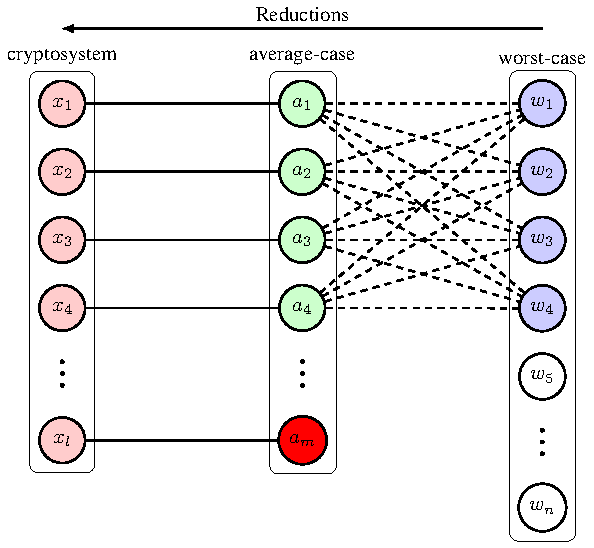
\includegraphics[page=1]{images/Lattice_crypto_tikz_folder.pdf}    
    \caption{A demonstration of a cryptosystem's computational security is based on an average-case problem. Each cryptographic instance $x_i$ corresponds to a random average-case instance $a_j$. Almost all random instances in the average-case problem can be mapped with the hard instances in a worst-case problem. There may be a fraction of average-case instances (colored in red) that can be solved easily, so their solutions entail solutions of the worst-case problem. But the fraction of such instances is negligible. The hard and easy instances in the worst-case problem are colored blue and white, respectively. The dashed lines indicate the worst-case to average-case reduction is random.}
    \label{fig:average2worst}
\end{figure}

The work by \citet{ajtai1996generating} served exactly this purpose by introducing the \textit{short integer solution} (SIS) problem and proving that SIS is an average-case problem with polynomial time reductions from three worst-case lattice problems to it. This work is knowably the first worst-case to average-case reduction. The significant implication of Ajtai's work in cryptography is the fact that it laid the foundation for the security of modern cryptosystems to be based on worst-case problems (via average-case problems). 
More importantly, this work sparked a number of important following up works including the learning with error and ring learning with error problems that advanced lattice-based cryptography to a new era. 





%\newpage
%\bibliography{references}
%\bibliographystyle{abbrvnat}

\end{document}